\documentclass[12pt]{article}

\usepackage[spanish]{babel}
\usepackage{hyperref}
\usepackage{graphicx}
\usepackage{listings}
\usepackage{color}
\usepackage{multicol}
\usepackage{amssymb}
\usepackage{enumitem}
\usepackage{here}
\usepackage{dsfont}
\usepackage{amsmath}
\usepackage{tipa}
\usepackage{float}
\spanishdecimal{.}

\title{Matemáticas para las Ciencias Aplicadas I}
\title{
	Tercera Lista de Problemas \\
	\textbf{Segunda  Parte} \\
	\vspace{1ex}
	\large Matemáticas para las Ciencias Aplicadas I \\
	Facultad de Ciencias, UNAM}

\date{\today}

\author{Flores Morán Julieta Melina \\ Zarco Romero José Antonio}

\begin{document}

\maketitle

%% De la sección 4.1: ejercicios 31, 57 y 71.
%% De la sección 4.2: ejercicios 31, 55 y 77.
%% De la sección 4.3: ejercicios 21, 36, 54 y 70.

%% 4.1 -----------------------------------------------------------------------------------------------------------------------------------------------------------------------------------------------------------------------------
\section{Sección 4.1 \\ Análisis De Funciones I: Aumento, Disminución Y Concavidad}
% 31 -------------------------------------------------------------------------------------------------------------
\subsection{Ejercicio 31} Flores Morán Julieta Melina \\

Encuentre: (a) los intervalos en los que $f$ aumenta, (b) los intervalos en los que $f$ disminuye, (c) los intervalos abiertos en los que $f$ es cóncava hacia arriba, (d) los intervalos abiertos en los que $f$ es cóncava hacia abajo, y (e) las coordenadas x de todos los puntos de inflexión.
\[
f(x) = \tan^{-1}(x^2-1)
\]

 Podemos determinar si f(x) crece o decrece en un intervalo según si su derivada es positiva o negativa en ese intervalo. Por esta razón, para determinar (a) y (b) primero necesitamos que derivar f(x).
  \begin{equation*}
  \begin{split}
    f'(x)
    &= \frac{d}{dx}(\tan^{-1}(x^2-1)) \\
    &= \frac{1}{1+(x^{2}-1)^{2}} \cdot \frac{d}{dx}((x^{2}-1)) \\
    &= \frac{1}{1+(x^{2}-1)^{2}} \cdot 2x \\
    \therefore
    f'(x)
    &= \frac{2x}{1+(x^{2}-1)^{2}}
  \end{split}
  \end{equation*}

  La derivada vale $0$ cuando $2x = 0$, es decir, cuando $x=0$. \\
   - Cuando $x>0$, $f'(x)>0$, es decir, es positiva y por lo tanto es creciente. \\
  - Cuando $x<0$, $f'(x)<0$, es decir, es negativa y por lo tanto es decreciente.\\

 \[
 \therefore
 \text{(a):  el intervalos en los que $f$ aumenta es} [0, \infty]
   \]
\[
  \text {(b):  el intervalos en los que $f$ decrece  es}  (-\infty, 0] \\
    \]

    Para responder a los últimos 3 incisos necesitamos información de la segunda derivada. Así que conviene calcularla.
     \begin{equation*}
  \begin{split}
    f''(x)
    &= \frac{d}{dx}( \frac{2x}{ 1+(x^{2}-1)^{2}  } )  \\
    &= \frac{  ( 1+(x^{2}-1)^{2}) \cdot  \frac{d}{dx} (2x) - \left[ 2x \cdot  \frac{d}{dx}   ( 1+(x^{2}-1)^{2})  \right]  }{ (1+(x^{2}-1)^{2} )^{2}  } \\
    &= \frac{  ( 1+(x^{2}-1)^{2}) \cdot  2 - \left[ 2x \cdot  \frac{d}{dx}   [(x^{2}-1)^{2}]  \right]  }{ (1+(x^{2}-1)^{2} )^{2}  } \\
    &= \frac{  2( 1+(x^{2}-1)^{2}) - \left[ 2x \cdot     2(x^{2}-1) \frac{d}{dx} (x^{2}-1)  \right]  }{ (1+(x^{2}-1)^{2} )^{2}  } \\
    &= \frac{  2( 1+(x^{2}-1)^{2}) - \left[ 2x \cdot     2(x^{2}-1) \cdot  2x  \right]  }{ (1+(x^{2}-1)^{2} ^{2}  } \\
    &= \frac{   2+2(x^{2}-1)^{2} - \left[ 8x^{2} \cdot(x^{2}-1)\right]  }{ (1+(x^{2}-1)^{2} )^{2}  } \\
    &= \frac{   2+2(x^{4}-2x^{2}+ 1) - \left[ 8x^{4} - 8x^{2}  \right]  }{ (1+(x^{2}-1)^{2} )^{2}  } \\
    &= \frac{   2+2x^{4}-4x^{2}+ 2 - 8x^{4} + 8x^{2}  }{ (1+(x^{2}-1)^{2} )^{2}  } \\
    &= \frac{-6x^{4} + 4x^{2} +4 }{ (1+(x^{2}-1)^{2} )^{2}  } \\
    \therefore
    f''(x)
    &= -2\frac{3x^{4} - 2x^{2} - 2 }{ (1+(x^{2}-1)^{2} )^{2}  } \\
  \end{split}
     \end{equation*}

     La concavidad depende del signo de $ f''(x)$. Para identificar estos intervalos primero conviene ubicar en que puntos $ f''(x) = 0$ , para reconocer más fácilmente $f''(x)<0$ y $f''(x)>0$·

\[ f''(x) = -2\frac{3x^{4} - 2x^{2} - 2 }{ (1+(x^{2}-1)^{2} )^{2}  } = 0  \]
\[ \iff \]
\[ 3x^{4} - 2x^{2} - 2 = 0 \]

Para calcular  $x$ más fácilmente sustituiremos la variable $x^{2}$ por t.

\[ 3t^{2} - 2t - 2 = 0 \]

Y usaremos la fórmula general.

 \begin{equation*}
  \begin{split}
    t
    &=  \frac{2 \pm \sqrt{4-4(3)(-2)} }{2(3)}  \\
    &=  \frac{2 \pm \sqrt{4+24} }{6}  \\
    &=  \frac{2 \pm \sqrt{28} }{6}  \\
    &=  \frac{2 \pm \sqrt{7 \cdot 4} }{6}  \\
    &=  \frac{2 \pm 2 \sqrt{7} }{6}  \\
    &=  \frac{1 \pm \sqrt{7} }{3}  \\
    \therefore
    x^{2}
    &= \pm \sqrt { \frac {1 \pm \sqrt { 7 } } { 3 }  } \\
  \end{split}
 \end{equation*}

Considerando que $1 -  \sqrt{7} \approx -1.64$, $x = \pm \sqrt {\frac{1 - \sqrt{7}}{3}}$ tiene raíces imaginarias.\\
Por lo tanto las raíces reales que nos interesan son
  \[
  x = \pm \sqrt {\frac{1 + \sqrt{7} }{3}} 
  \]
Estos son los puntos de inflexión, donde $f(x) = 0$. Así que evaluaremos cada intervalo que nos es de interés,para conocer el signo de $ f''(x) $. Donde es negativa, es cóncava hacia abajo y donde es positiva es cóncava hacia arriba.
  
\begin{table}[h]
\centering
\begin{tabular}{|c|c|c|}
\hline
Intervalo &  Signo de $f''(x)$ & concavidad hacia \\
\hline
$(-\infty, -\sqrt{\frac{1 + \sqrt{7}}{3}})$ & - & abajo\\
\hline
$(-\sqrt{\frac{1 + \sqrt{7}}{3}}, \sqrt{\frac{1 + \sqrt{7}}{3}})$ & + & arriba \\
\hline
$(\sqrt{\frac{1 + \sqrt{7}}{3}}, \infty)$ & - & abajo \\
\hline
\end{tabular}
\end{table}

 \[
 \therefore
 \text{(c):  el intervalos  en los que $f$ es cóncava hacia arriba } (-\sqrt{\frac{1 + \sqrt{7}}{3}}, \sqrt{\frac{1 + \sqrt{7}}{3}})
   \]
\[
  \text {(d):  los  intervalos en los que $f$  es cóncava hacia abajo  son }  (\sqrt{\frac{1 + \sqrt{7}}{3}}, \infty) \text{ y } (-\infty, -\sqrt{\frac{1 + \sqrt{7}}{3}})

    \]
\[
  \text {(e): las coordenadas x de todos los puntos de inflexión son }  x =  \sqrt {\frac{1 + \sqrt{7} }{3}}  \text{ y }  x = - \sqrt {\frac{1 + \sqrt{7} }{3}} 

    \]
% 57 -------------------------------------------------------------------------------------------------------------
\subsection{Ejercicio 57} Zarco Romero José Antonio \\

\begin{enumerate}[label=(\alph*)]
\item Demuestre que un polinomio cúbico general
  \[
  f(x) = ax^3 + bx^2 + cx + d \qquad (a\neq 0)
  \]
  tiene exactamente un punto de inflexión.

  Calculando las dos primeras derivadas de $f$ obtenemos
  \begin{align*}
    f'(x)
    &= 3ax^2 + 2bx +c \\
    f''(x)
    &= 6ax +2b \\
    &= 6a\left(x+\frac{b}{3a}\right)
  \end{align*}
  Ahora, calculamos cuando ocurre $f''(x)=0$
  \begin{align*}
    6a\left(x+\frac{b}{3a}\right)
    &= 0\\
    x+\frac{b}{3a}
    &= 0 \\
    x
    &= -\frac{b}{3a}
  \end{align*}
  Así, conocemos entonces que $f$ cambia su dirección de concavidad en $x=-\frac{b}{3a}$. \\ 
  $\therefore -\frac{b}{3a}$ es el único un punto de inflexión.
  \
  \begin{flushright}
    $\blacksquare$
  \end{flushright}

\item Demuestre que si un polinomio cúbico tiene tres intersecciones en el eje $x$, entonces el punto de inflexión ocurre en el valor promedio de las intersecciones.

  Si $f(x)$ tiene 3 intersecciones con el eje $x$, entonces podemos expresarlo como
  \[
  f(x)=a(x-r_1​)(x-r_2​)(x-r_3​)
  \]
  donde $r_1,r_2$ y $r_3​$ son las raíces del polinomio.
  
  Si desarrollamos la ecuación anterior, también se puede expresar como
  \begin{align*}
    & a(x-r_1​)(x-r_2​)(x-r_3​) \\
    & = a(x^2-r_1x-r_2x+r_1r_2)(x-r_3) \\
    & = a(x^3-r_1x^2-r_2x^2+r_1r_2x-r_3x^2+r_1r_3x+r_2r_3x-r_1r_2r_3) \\
    & = a[x^3-(r_1+r_2+r_3)x^2+(r_1+r_2+r_3)x-r_1r_2r_3]
  \end{align*}

  Comparando términos con $ax^3 + bx^2 + cx + d$, se sigue que $b=-a(r_1+r_2+r_3)$. De este modo, al sustituir el valor de $b$ en el punto de inflexión $-\frac{b}{3a}$, tenemos que
  \[
  -\frac{b}{3a}= -\frac{-a(r_1+r_2+r_3)}{3a}=\frac{1}{3}(r_1+r_2+r_3)
  \]
  $\therefore $ El punto de inflexión ocurre en el valor promedio de las intersecciones
  \begin{flushright}
    $\blacksquare$
  \end{flushright}


\item Utilice el resultado del inciso (b) para encontrar el punto de inflexión del polinomio cúbico $f(x) = x^3-3x^2 + 2x$, y verifique su resultado usando $f''$ para determinar dónde $f$ es cóncava hacia arriba y cóncava hacia abajo.

  Primero, debemos reescribir $f(x)$
  \begin{align*}
    f(x)
    &= x^3-3x^2 + 2x\\
    &=x(x^2-3x+2)\\
    &=x(x-1)(x-2)
  \end{align*}
  donde las raíces del polinomio son $r_1=0,r_2=1$ y $r_3=2$. Sustituyendo estos valores en el resultado del inciso (b), tenemos que el punto de inflexión es igual a
  \begin{align*}
    \frac{1}{3}(r_1+r_2+r_3)
    &= \frac{1}{3}(0+1+2) \\
    &= \frac{1}{3}(3) \\
    &= 1
  \end{align*}
  Por lo que 1 es el punto de inflexión.

  Para verificar el resultado, calculamos las dos primeras derivadas de $f$ donde obtenemos que
  \begin{align*}
    f'(x)
    &= 3x^2 - 6x +2\\
    f''(x)
    &= 6x -6 \\
    &= 6 (x-1)
  \end{align*}
  Así, comprobamos que 1 es el punto de inflexión, pues es cuando $f''(x)=0$. Procedemos a tabular
  \begin{table}[H]
    \centering
    \begin{tabular}{c|c|c}
      \hline
      Intervalo & $f''(x) = 6(x-1)$ & Conclusión \\
      \hline
      $-\infty<x<1$ & - & $f$ es cóncava hacia abajo \\
      $1<x<-\infty$ & + & $f$ es cóncava hacia arriba \\
      \hline
    \end{tabular}
  \end{table}
  $\therefore $ El punto de inflexión es (1,0), $f$ es cóncava hacia arriba en el intervalo $(1,+\infty)$ y cóncava hacia abajo en el intervalo $(-\infty,1)$.
  
\end{enumerate}

% 71 -------------------------------------------------------------------------------------------------------------
\subsection{Ejercicio 71} Flores Morán Julieta Melina \\

Suponiendo que $A, k$ y $L$ son constantes positivas, verifique que la gráfica de $y=L/(1+Ae^{-kt})$ tiene un punto de inflexión en $\left( \frac{1}{k}\ln{A},\frac{1}{2}L \right)$. \\
La fórmula dada es la función que describe el crecimiento de curvas logísticas. Para conocer los puntos de inflexión, necesitamos conocer la segunda derivada con respecto a t. Si multiplicamos ambos lados de la fórmula por $e^{kt}(1+Ae^{-kt})$, obtenemos:
\[
ye^{kt}(1+Ae^{-kt}) = Le^{kt}
\]
\[
ye^{kt}+yAe^{kt}e^{-kt} =Le^{kt}
\]
\[
ye^{kt}+yAe^{kt-kt} = Le^{kt}
\]
\[
ye^{kt}+yAe^{0} = Le^{kt}
\]
\[
ye^{kt}+yA = Le^{kt}
\]
Y usando derivación implícita podemos obtener:
\[
\frac{d}{dt}[y(e^{kt}+A)] = \frac{d}{dt} (Le^{kt})
\]
\[
y \frac{d}{dt}e^{kt} +  (e^{kt}+A)\frac{dy}{dt} = L\frac{d}{dt}(e^{kt})
\]
\[
yke^{kt} +  (e^{kt}+A)\frac{dy}{dt} = Lke^{kt}
\]
\[
  (e^{kt}+A)\frac{dy}{dt} = Lke^{kt} -yke^{kt} 
\]
\[
 \frac{dy}{dt} = \frac{ ke^{kt} (L-y) } {e^{kt}+A}
 \]
 \[
 \frac{dy}{dt} = \frac{ ke^{kt} (L-y) } {Le^{kt}/y} 
 \]
 \[
 \frac{dy}{dt} = \frac{K} {L} y(L-y) 
 \]
 Necesitamos la segunda derivada.
 \[
\frac{d^{2}y}{dt^{2}}} = \frac{dy}{dt} \left[\frac{K} {L} y(L-y)  \right]
  \]
   \[
   \frac{d^{2}y}{dt^{2}}} =\frac{K} {L} \left[  y\frac{d}{dt}(L-y) +(L-yy \frac{dy}{dt}  \right]
     \]
 \[
 \frac{d^{2}y}{dt^{2}}} =\frac{K} {L} \left[  (y)(-\frac{dy}{dt)
     }) +(L-y)  \frac{dy}{dt}  \right]
   \]
  \[
 \frac{d^{2}y}{dt^{2}}} =\frac{K} {L} \left[  (y)(-[\frac{K} {L} y(L-y) ]
     }) +(L-y)  \frac{K} {L} y(L-y)   \right]
     \]
 \[
 \frac{d^{2}y}{dt^{2}}} =\frac{K} {L} \left[ - y^{2}\frac{K} {L}(L-y) 
 +(L-y)^{2}  \frac{K} {L} y   \right]
   \]

 \[
 \frac{d^{2}y}{dt^{2}}} =\frac{K^2} {L^2} y (L-y)(L-2y)
 \]

 Para la curva logística ocurre que k>0, y>0 y L-y>0. Así que la segunda derivada solo cambia de signo si L-2y cambia de signo.
 Si L-2y >0, entonces f''(x) >0.  Si L-2y <0, entonces f''(x) <0.
 Entonces la gráfica de y en el tiempo es cóncava hacia arriba si y<L/2, y cóncava hacia abajo si y>L/2, y tienen un punto de inflexión en y=L/2 ya que este cambio de signos ocurre.
 Para saber la coordenada en el eje x, remplazamos

  \[
 \frac{L}{2} =\frac{L} {1+Ae^{-kt} 
   \]
    \[
 \frac{L}{2} =\frac{L} {1+Ae^{-kt} }
   \]
     \[
1  =1+Ae^{-kt}
  \]
  \[
t = \frac{1}{K} \ln{A}} = \frac{lnA}{k}
   \]
%% 4.2 -----------------------------------------------------------------------------------------------------------------------------------------------------------------------------------------------------------------------------
\section{Sección 4.2 \\ Análisis De Funciones II: Extremos Relativos; Graficar Polinomios} 
% 31 -------------------------------------------------------------------------------------------------------------
\subsection{Ejercicio 31} Zarco Romero José Antonio \\

Utilice la derivada dada para encontrar todos los puntos críticos de $f$ y en cada punto crítico determine si ocurre un máximo relativo, un mínimo relativo o ninguno de los dos. Supongamos en cada caso que $f$ es continua en todas partes.
\[
f'(x)=\ln{\left( \frac{2}{1+x^2} \right)}
\]

Al establecer $1+x^2=0$ se obtiene que $x=\pm 1$, por tanto -1 y 1 son puntos críticos
  \begin{table}[H]
    \centering
    \begin{tabular}{c|c|c}
      \hline
      Intervalo & $f'(x) = \ln{\left( \frac{2}{1+x^2} \right)$ & Conclusión \\
      \hline
      $(-\infty,-1)$ & - & $f$ es decreciente \\
      $(-1,1)$ & + & $f$ es creciente\\
      $(1,+\infty)$ & - & $f$ es decreciente\\
      \hline
    \end{tabular}
  \end{table}
  Dado que el signo de $f'$ cambia de - a + en $x=-1$, hay un mínimo relativo allí, y
  dado que el signo de $f'$ cambia de + a - en $x=1$, hay un máximo relativo allí.

  $\therefore $ Los puntos críticos son -1 y 1, en -1 ocurre un mínimo relativo y en 1 un máximo relativo.

% 55 -------------------------------------------------------------------------------------------------------------
\subsection{Ejercicio 55} Flores Morán Julieta Melina \\

Haz una gráfica del polinomio y etiqueta las coordenadas de las intersecciones, los puntos estacionarios y los puntos de inflexión. Comprueba tu trabajo con una utilidad gráfica.
\[
p(x) = (x + 1)^2 (2x-x^2 )
\]
Primero, podemos calcular las intersecciones con los ejes. \\
\textbf {Intersecciones con el eje x:}
\[
p(x) = (x + 1)^2 (2x-x^2 ) = 0 \iff 
\]
\[
x+1 = 0 \iff  x = -1 \text{ o } 
 \]
 \[
 2x-x^{2}=0 \iff x = 0, 2
 \]
 Por lo que los puntos de intersección con x son:
 \[
(0,0), (2,0), (-1, 0)
 \]
 Donde -1 es un raíz con una multiplicidad de 2, entonces la gráfica de p(x) será tangente al eje x en x=-1, pero no lo cruzara y no habrá un punto de inflexión aquí. 0 y 2 tienen multiplicidad simple, por lo que la grafica no es tangente al eje x en x=0 y x=2, cruza el eje x ahí y puede o no tener un punto de inflexión aquí.\\
 -Intersección con el eje y:\\
 \[
 p(0) = (0 + 1)^2 (2\cdot0-0^2) = 0
 \]
 
 La intersección en el eje y se da en (0,0).\\
\textbf  {Puntos estacionarios:}\\
 Los puntos estacionarios se dan cuando p'(x) = 0.\\
 Para saber esto, necesitamos primero calcular p'(x).\\
 \begin{equation*}
  \begin{split}
    p'(x)
    &=  \frac{d} {dx} \left[ (x + 1)^2 (2x-x^2)\right]  \\
    &=   (x + 1)^2  \frac{d} {dx}(2x-x^2) + (2x-x^2) \frac{d} {dx} (x + 1)^2  \\
    &=   (x + 1)^2 (2-2x) + (2x-x^2)  2(x + 1)  \\
    &=   (x + 1) \left(  (x + 1) (2-2x)  +  2(2x-x^2)  \right) \\
    &=   (x + 1) \left(  2x-2x^{2}+2-2x  +  4x-2x^2  \right) \\
    \therefore
    p'(x)
    &=    (x + 1)\left(  -4x^{2} +4x+2\right) \\ \\
  \end{split}
 \end{equation*}


 \[
  p'(x) =    (x + 1)\left(  -4x^{2} +4x+2\right) = 0
  \]
  \[
  \iff
  \]
   \[
  x + 1  = 0 \iff x =-1
  \]
   \[
 -4x^{2} +4x+2  = 0 \iff x = \frac{1 \pm \sqrt{3} }{2}
 \]
 Evaluando estos puntos:
 \[
  p(-1) = \left( -1 + 1 \right)^2 \left(2\left( -1 \right)- \left(-1 \right) ^2 \right) = 0
  \]
 \[
  p(\frac{1 + \sqrt{3} }{2}) = \left( \left( \frac{1 + \sqrt{3} }{2}\right) + 1 \right)^2 \left(2\left( \frac{1 + \sqrt{3} }{2} \right)- \left( \frac{1 + \sqrt{3} }{2} \right) ^2 \right) = \frac{9+6\sqrt{3}}{4}
  \]
   \[
  p(\frac{1 - \sqrt{3} }{2}) = \left( \left( \frac{1 - \sqrt{3} }{2}\right) + 1 \right)^2 \left(2\left( \frac{1 - \sqrt{3} }{2} \right)- \left( \frac{1 - \sqrt{3} }{2} \right) ^2 \right) = \frac{9-6\sqrt{3}}{4}
  \]
    Por esto, los puntos estacionarios son:
    \[
    \left(-1,  0\right) \text{, } 
\left(\frac{1 + \sqrt{3} }{2},  \frac{9+6\sqrt{3}}{4}\right) \text{  y  }
\left( \frac{1 - \sqrt{3} }{2}, \frac{9-6\sqrt{3}}{4} \right)
\]
Estos puntos pueden ser puntos de inflexión o extremos relativos.
Son extremos relativos si p' cambia de signo, como es el caso, además podemos aprovechar para evaluar si la función que queremos es creciente o decreciente en el intervalo, como podemos observar:
  \begin{table}[H]
    \centering
    \begin{tabular}{c|c|c}
      \hline
      Intervalo & $p'(x) = (x + 1)\left(  -4x^{2} +4x+2\right)\right)$ & Conclusión \\
      \hline
      $(-\infty, -1)$ & + & creciente \\
      $(-1, \frac{1 - \sqrt{3} }{2} )$ & - & decreciente \\
      $( \frac{1 - \sqrt{3} }{2} , \frac{1 + \sqrt{3} }{2} )$ & + & creciente\\
      $( \frac{1 + \sqrt{3} }{2} ,+\infty)$ & - & decreciente\\
      \hline
    \end{tabular}
  \end{table}
  Como podemos observar, la derivada cambia de signo en $-1$, $\frac{1 - \sqrt{3}}{2}$ y $\frac{1 + \sqrt{3} }{2}$. Por lo que los 3 puntos  son extremos relativos. Para saber si son máximos o mínimos debemos observar como cambian los signos.\\
Para $-1$, a su izquierda $p'(x)<0$ y a su derecha $p'(x)<0$ por lo que es un máximo relativo.\\
Para  $ \frac{1 - \sqrt{3}}{2}$ , a su izquierda $p'(x)<0$ y a su derecha $p'(x)>0$ por lo que es un mínimo relativo.\\
Para  $\frac{1 + \sqrt{3} }{2} $ , a su izquierda $p'(x)>0$ y a su derecha $p'(x)<0$ por lo que es un máximo relativo.    
    \\
\textbf{Puntos de inflexión:}\\
Los puntos de inflexión son los puntos donde la segunda derivada es 0. Para esto necesitamos calcular p''(x).
 \begin{equation*}
  \begin{split}
    p''(x)
    &=  \frac{d} {dx} \left[  (x + 1)\left(  -4x^{2} +4x+2\right) ]  \\
    &=  (x+1) \frac{d} {dx} (-4x^{2} +4x+2) + (-4x^{2} +4x+2) \frac{d} {dx} (x + 1)\\
    &=  (x+1)  (-8x +4) + (-4x^{2} +4x+2) \\
    &=  -8x^{2} +4x -8x +4-4x^{2} +4x+2 \\
    \therefore
    p''(x)
    &=  -12x^{2} +6 \\
  \end{split}
 \end{equation*}
 Los puntos de inflexión son en donde se cumple que:
 \[
-12x^{2} +6  = 0 
 \]
  \[
\iff
\]
 \[
x = \pm \frac{\sqrt{2}}{2}
\]
Evaluando los puntos:
 \[
  p(\frac{\sqrt{2}}{2}) = \left( \left( \frac{\sqrt{2}}{2} \right) + 1 \right)^2 \left(2\left( \frac{\sqrt{2}}{2}  \right)- \left(\frac{\sqrt{2}}{2}  \right) ^2 \right) = \frac{5}{4} + \sqrt{2}
  \]
 \[
  p(\frac{-\sqrt{2}}{2}) = \left( \left( \frac{-\sqrt{2}}{2} \right) + 1 \right)^2 \left(2\left( \frac{-\sqrt{2}}{2}  \right)- \left(\frac{-\sqrt{2}}{2}  \right) ^2 \right) = \frac{5}{4} - \sqrt{2}
  \]
   Por esto, los puntos de inflexión son:
  \[
\left(\frac {\sqrt{2}}{2},   \frac{5}{4} + \sqrt{2} \right) } \text{  y  }
\left(-\frac {\sqrt{2}}{2},  \frac{5}{4} - \sqrt{2} \right)
\]
Podemos evaluar como cambia la concavidad en estos puntos evaluando el signo de $p''(x)$.
  \begin{table}[H]
    \centering
    \begin{tabular}{c|c|c}
      \hline
      Intervalo & $p''(x) = -12x^{2} +6 $ & Concavidad hacia \\
      \hline
      $(-\infty, -\frac{\sqrt{2}}{2})$ & - & abajo  \\
      $( -\frac{\sqrt{2}}{2}, \frac{\sqrt{2}}{2} )$ & + & arriba \\
      $( \frac{\sqrt{2}}{2} , +\infty )$ & - & abajo \\
      \hline
    \end{tabular}
  \end{table}

  Con esta información, una aproximación de la gráfica puede ser:
  \begin{figure}[H]
\centering
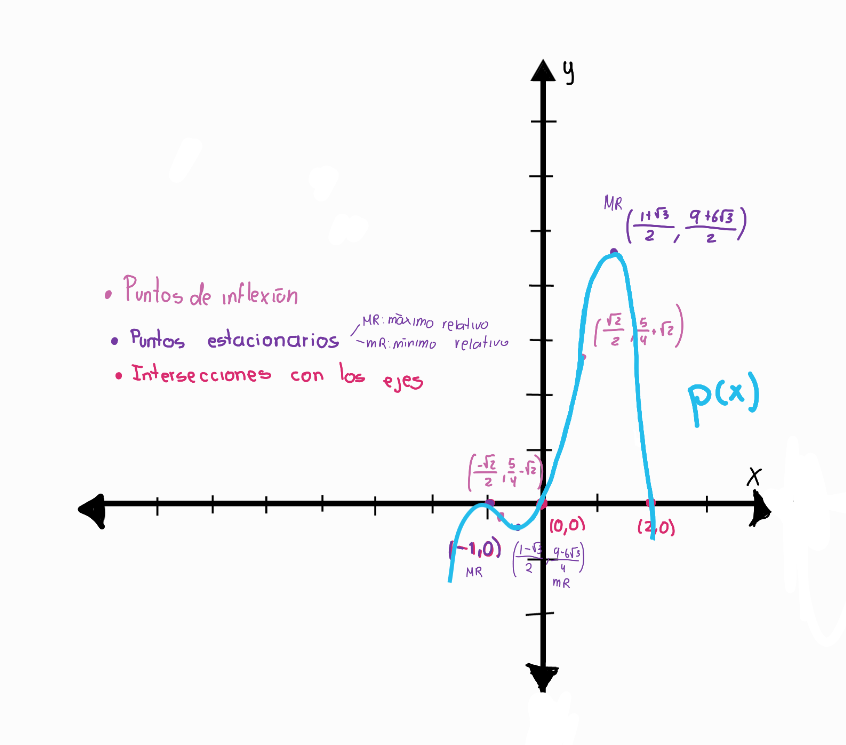
\includegraphics[width=0.4\textwidth]{../img/img_Lista3/grafica55.png}
  \end{figure}
  Mientras que en una utilidad gráfica se visualiza de la siguiente forma:
  \begin{figure}[H]
\centering
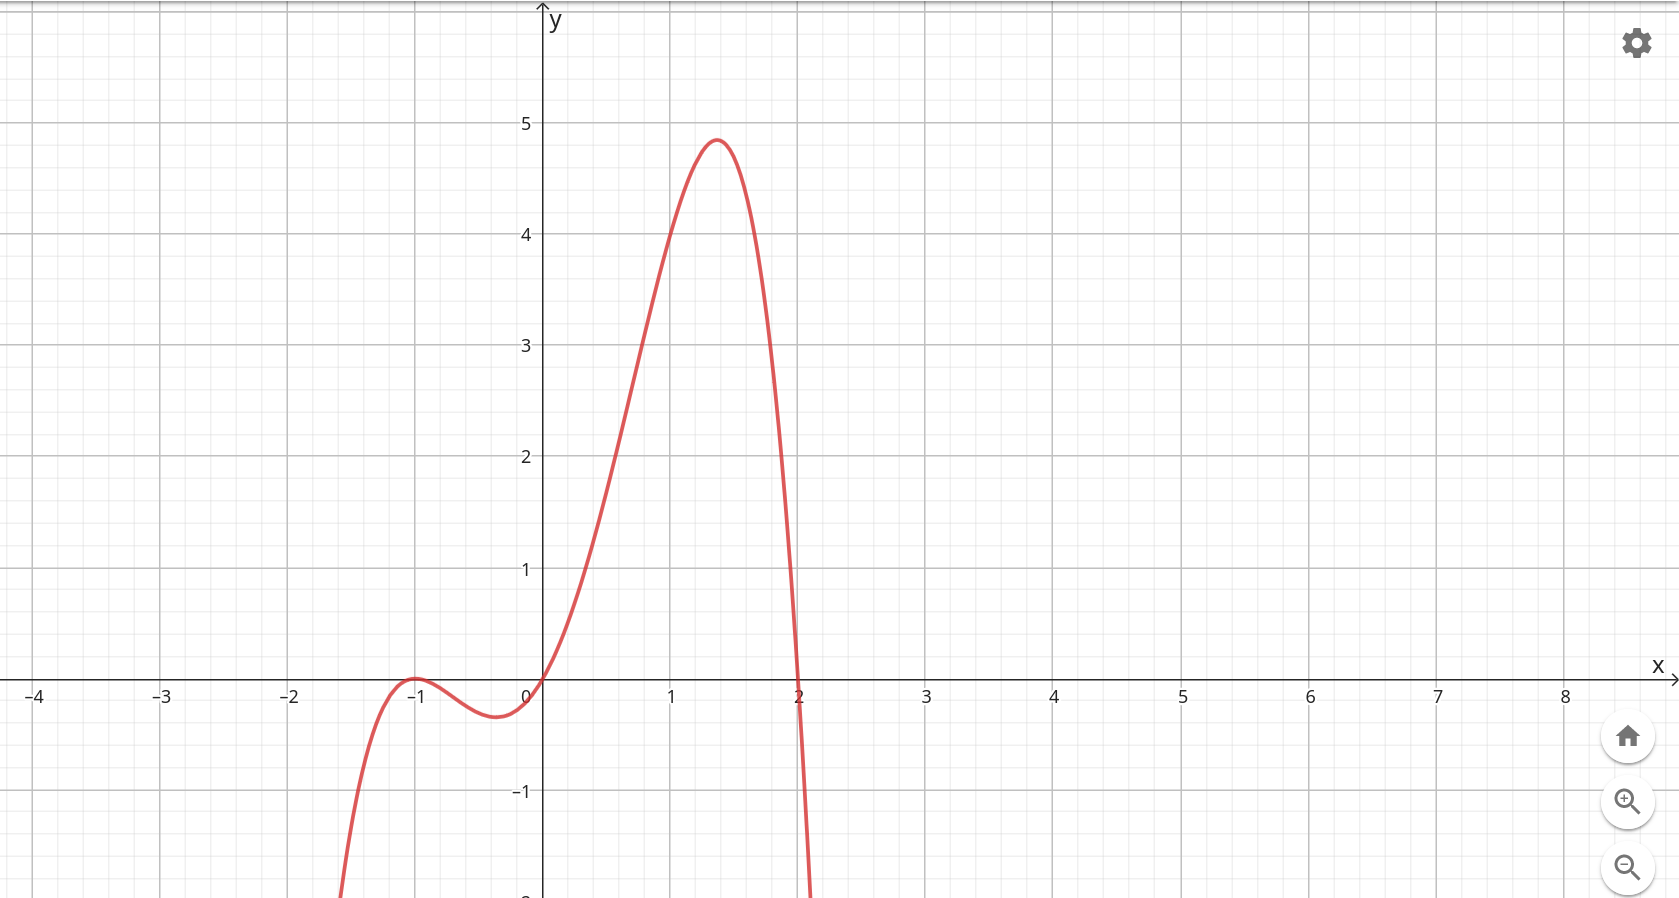
\includegraphics[width=0.4\textwidth]{../img/img_Lista3/grafica255.png}
  \end{figure}
% 77 -------------------------------------------------------------------------------------------------------------
\subsection{Ejercicio 77} Zarco Romero José Antonio \\

En cada parte, encuentre $k$ de modo que $f$ tenga un extremo relativo en el punto donde $x = 3$.
\begin{enumerate}[label=(\alph*)]
\item $f(x)=x^2+\frac{k}{x}$

  Calculando la primera derivada de $f$ obtenemos que
  \begin{align*}
    f'(x)
    &= 2x-\frac{k}{x^2} \\
    & = \frac{2x^3-k}{x^2}
  \end{align*}
  Cuando $f'(x)=0$, tenemos que
  \begin{align*}
    \frac{2x^3-k}{x^2}
    &=0\\
    2x^3-k
    &=0\\
    k
    &=2x^3\\
    k\vline_{x=3}
    &= 2(3)^3\\
    &=54
  \end{align*}
  $\therefore k=54$

\item $f(x)=\frac{x}{x^2+k}$
  

  Calculando la primera derivada de $f$ obtenemos que
  \begin{align*}
    f'(x)
    &= \frac{x^2+k-2x^2}{(x^2+k)^2}\\
    &= \frac{k-x^2}{(x^2+k)^2}
  \end{align*}
  Cuando $f'(x)=0$, tenemos que
  \begin{align*}
    \frac{k-x^2}{(x^2+k)^2}
    &=0\\
    k-x^2
    &=0\\
    k
    &=x^2\\
    k\vline_{x=3}
    &= (3)^2\\
    &=9
  \end{align*}
  $\therefore k=9$
\end{enumerate}

%% 4.3 -----------------------------------------------------------------------------------------------------------------------------------------------------------------------------------------------------------------------------
\section{Sección 4.3 \\  Análisis De Funciones III: Funciones Racionales, Cúspides Y Tangentes Verticales}
% 21 -------------------------------------------------------------------------------------------------------------
\subsection{Ejercicio 21} Flores Morán Julieta Melina \\

Dibuja una gráfica de la función racional y etiqueta las coordenadas de los puntos estacionarios y los puntos de inflexión. Muestra las asíntotas horizontales, verticales, oblicuas y curvilíneas y etiquetarlas con sus ecuaciones. Etiquete los puntos, si los hay, donde la gráfica cruza una asíntota. Comprueba tu trabajo con una utilidad gráfica.
\[
f(x)= \frac{(x-2)^3}{x^2}
\]
\textbf{Puntos estacionarios:}\\
Estos puntos los encontramos igualando $f'(x) = 0$.
Necesitamos calcular la derivada:\\
\begin{align*}
  $f'(x)$
  &= \frac{d}{dx} \left[ \frac{(x-2)^3} {x^2} \right] \\
   &= \frac{x^{2} \frac{d}{dx}(x-2)^3 - \left[ (x-2)^3  \frac{d}{dx}(x^{2}) \right] } {x^4}\\
  &= \frac{x^{2} 3(x-2)^2 - \left[ (x-2)^3  2x \right] } {x^4} \\
    &= \frac{x^{2} 3(x^2-4x+4) - \left[ x^{3} - 6 x^{2} + 12x-8  (2x)  \right] }  {x^{4}}\\
  &= \frac { 3x^{4}-12x^{3}+12x^{2} - \left[  2x^{4} - 12 x^{3} + 24x^{2}-16x \right] } {x^{4}}\\
  &= \frac { 3x^{4}-12x^{3}+12x^{2} -  2x^{4} + 12 x^{3} - 24x^{2} + 16x } {x^{4}}\\
  &= \frac {x^{4}-12x^{2}+16x} {x^{4}}\\
  &= \frac {x^{3}-12x +16}  {x^{3}}\\
  &= \frac {x^{3}-12x+16}  {x^{3}}\\
\end{align*}
Igualamos a 0:
\[
f'(x)  =  \frac {x^{3}-12x+16}  {x^{3}} = 0
\]
\[
\iff
\]
\[
 x^{3}-12x+16 = 0
 \]
 Pero para encontrar los valores de x nos será de utilidad factorizar.
 \[
 x^{3}-12x+16 =  x^{3}-16x +4x+16  = x(x-4) (x+4) + 4(x+4) = (x+4) (x-2)^{2}
 \]
 Entonces
 \[
 (x+4) (x-2)^{2} = 0 
 \]
\[
\iff
\]
\[
  x+4 = 0 \iff x = -4 
 \]
\[
   (x-2)^{2} = 0 \iff x =2 
\]
Y evaluando los puntos:
\[
f(-4) =  \frac{(-4-2)^3}{(-4)^2} = \frac{(-6)^3}{16} = \frac{-216}{16} =-13.5
\]
\[
f(2) =  \frac{(2-2)^3}{2^2} = \frac{(2-2)^3}{2^2} =  \frac{0}{4} = 0
\]
Entonces los puntos estacionarios son :
\[
\left( -4, -13.5\right) \text{ y } \left( 2, 0\right)
\]
\textbf{Puntos de inflexión}\\
Estos los encontraremos igualando $f''(x) = 0$. Entonces, necesitamos calcular $f''(x)$.
\begin{align*}
  $f''(x)$
  &= \frac{d}{dx} \left[  \frac {x^{3}-12x+16}  {x^{3}} \right] \\
  &=   \frac {x^{3} \frac{d}{dx} (x^{3}-12x+16) - \left[ \frac{d}{dx}(x^{3}) (x^{3}-12x+16)  \right] }  {x^{6}}  \\
  &=   \frac {x^{3} (3x^{2}-12) - \left[(3x^{2})(x^{3}-12x+16)  \right] }  {x^{6}}  \\
  &=   \frac { 3x^{5}-12x^{3} - \left[3x^{5}-36x^{3}+48x^{2} \right] }  {x^{6}}  \\
  &=   \frac { 3x^{5}-12x^{3} - 3x^{5}+36x^{3}-48x^{2}}  {x^{6}}  \\
  &=   \frac { 24x^{3}-48x^{2}}{x^{6}}  \\
  &=   \frac { x^{2} (24x-48)} {x^{6}}  \\
  &=   \frac { 24x-48} {x^{4}}  \\
  &=   \frac { 24 (x-2)} {x^{4}}  \\
\end{align*}
Igualando $f''(x) = 0$
\[
\frac { 24 (x-2)} {x^{4}}  = 0
\]
\[
\iff
\]
\[
 24 (x-2)  = 0 \iff (x-2) = 0 \iff x = 2
 \]
 Entonces el punto de inflexión es:
 \[
\left( 2, 0 \right)
\]
\textbf{Asíntotas:}\\
-Horizontales: Ya que el grado de numerador es 3 y es más grande que el del denominador, no tiene asíntota horizontal.\\
-Verticales: La función se indefine únicamente cuando $x^{2} = 0$, por lo que hay una asíntota horizontal en x = 0. \\
-Oblicuas: Ya que el numerador es de un grado mayor que el denominador, podemos buscar este tipo de asíntota reescribiendo la fórmula dada.
\begin{align*}
  $f(x)$
  &= \frac{(x-2)^3}{x^2} \\
  &=  \frac{x^{3}-6x^{2} + 12x - 8}{x^2} \\
  &=  \frac{x^{3}}{x^2} -  \frac{6x^{2}}{x^2} + \frac{12x-8}{x^2}\\
   &=  x  - 6 + \frac{12x-8}{x^2}\\
\end{align*}
Ya que el grado del nuevo numerador es menor que la del denominador, y=x-6 es una asíntota. Ya que en la fórmula original el numerador solo excedía en uno a el denominador, es una asíntota oblicua, $y =x-6$ es una línea.
-Curvilíneas: En este caso, el denominador solo era menor en una unidad al numerador y para que existan este tipo de asíntotas deber ser menor en dos unidades o más; por lo que no hay asíntotas curvilíneas.

\textbf{Puntos donde la gráfica intersecta una asíntota}:\\
Tenemos dos asíntotas, en la asíntota vertical no puede existir tal cruce ya que la función evaluada en x = 0 esta indeterminada.
En cuanto la asíntota oblicua podemos buscar una intersección entre $y =x-6$ y y= $\frac{(x-2)^3}{x^2} $
Esto lo podemos encontrar igualando
\begin{align*}
  x- 6= \frac{(x-2)^3}{x^2}\\
  x-6 = x  - 6 + \frac{12x-8}{x^2}\\
  0 = \frac{12x-8}{x^2}\\
  0 = 12x-8\\
  8 = 12x\\
  \frac{8}{12} = x\\
  x = \frac{2}{3} \\
\end{align*}
Una vez conociendo x, podemos buscar y
\begin{align*}
 y = x-6\\
 y =  \frac{2}{3} - \frac{18}{3}
 y= \frac{-16}{3}
\end{align*}
Entonces el punto de intersección es $\left( \frac{2}{3} , -\frac{16}{3}  \right)$\\
Con esta información, podemos crear un esbozo de la gráfica.\\
\begin{figure}[H]
\centering
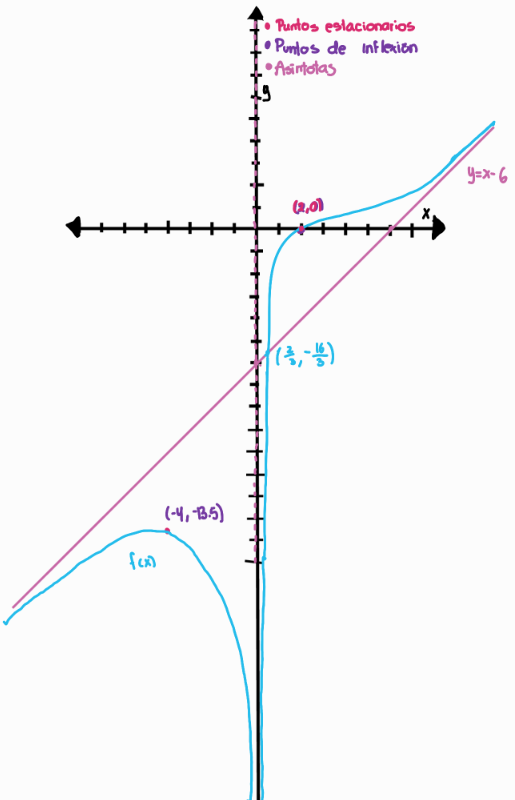
\includegraphics[width=0.4\textwidth]{../img/img_Lista3/21_2.png}
\end{figure}
\\
Y podemos compararla por la creada por una utilidad gráfica.\\
\begin{figure}[H]
\centering
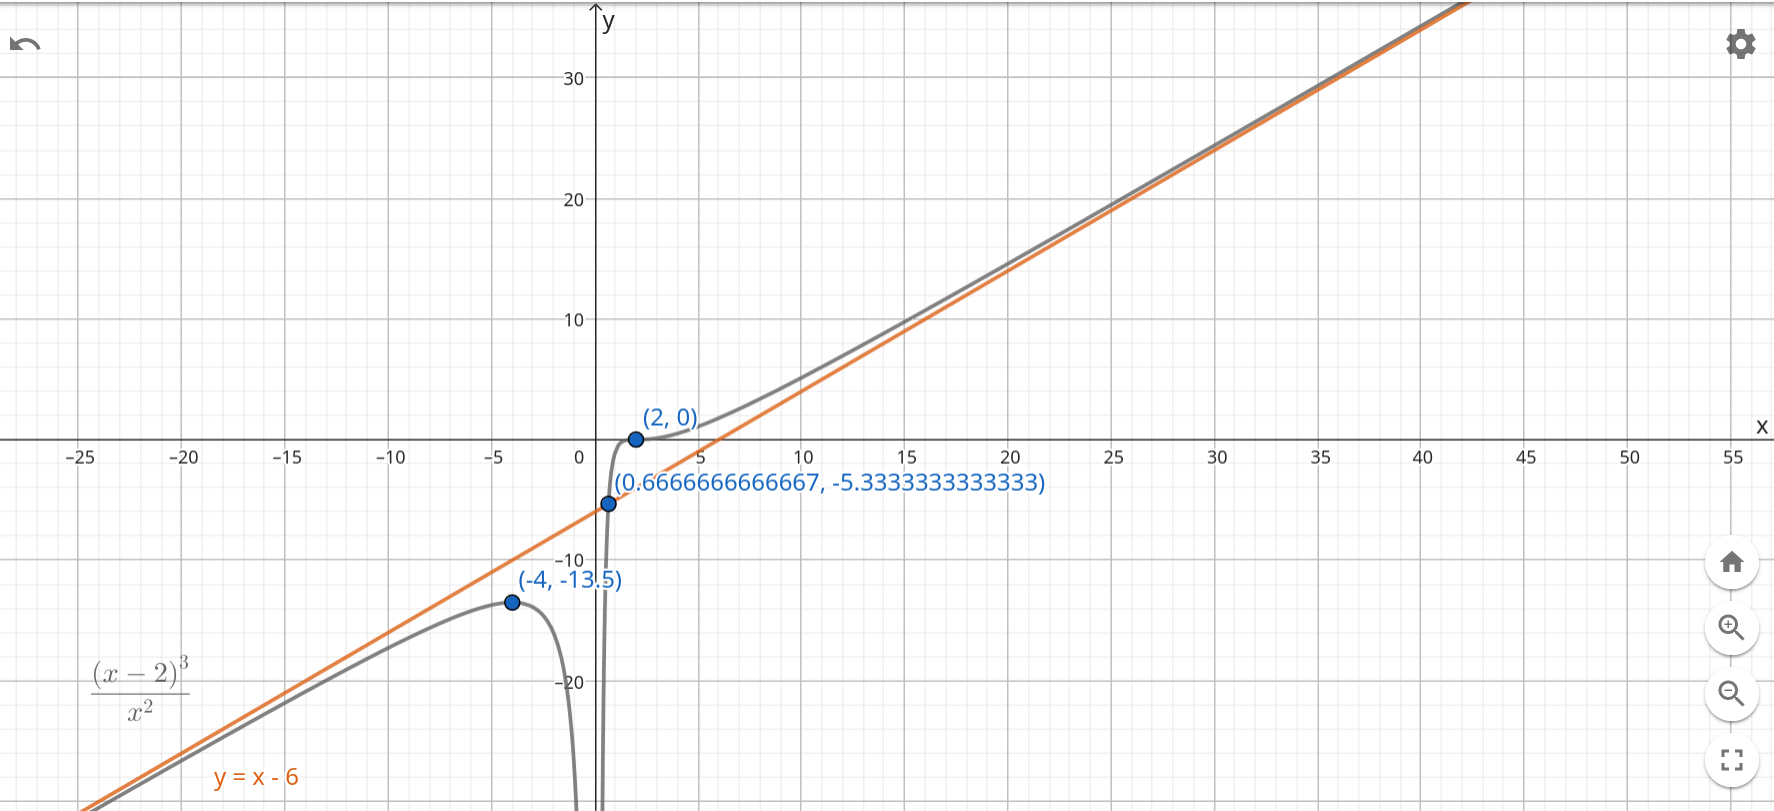
\includegraphics[width=0.4\textwidth]{../img/img_Lista3/21_1.png}
\end{figure}
% 36 -------------------------------------------------------------------------------------------------------------
\subsection{Ejercicio 36} Zarco Romero José Antonio \\

Dé una gráfica de la función e identifique las ubicaciones de todos los puntos críticos y puntos de inflexión. Comprueba tu trabajo con una utilidad gráfica.
\[
5x^{2/3}+x^{5/3}
\]

Nos ayudará en nuestro análisis escribir
\[f(x)=5x^{2/3}+x^{5/3}=x^{2/3}(5+x)\]
\begin{itemize}
\item \textbf{Simetría}: No existen simetrías sobre los ejes de coordenadas ni sobre el origen.
\item \textbf{Intersecciones $x$ y $y$}: Al establecer $x^{2/3}(5+x)=0$ se obtienen las intersecciones $x=0,-5$. También, establecer $x=0$ produce la intersección con el eje $y$ en $y=0$.
\item  \textbf{Asíntotas verticales}: Ninguna, ya que $f(x) = 5x^{2/3}+x^{5/3}$ es continua en todas partes.
\item  \textbf{Comportamiento final}: 
  \begin{align*}
    \lim_{x \to +\infty}5x^{2/3}+x^{5/3} = \lim_{x \to +\infty} x^{2/3}(5+x) = +\infty \\
    \lim_{x \to -\infty} 5x^{2/3}+x^{5/3} = \lim_{x \to -\infty}  x^{2/3}(5+x) = -\infty 
  \end{align*}
\item \textbf{Derivadas}:
  \begin{align*}
    \frac{dy}{dx}
    &= f'(x) = \frac{10}{3}x^{-1/3} + \frac{5}{3}x^{2/3} = \frac{5}{3}x^{-1/3}(2+x)\\
    &= \frac{5(x+2)}{3x^{1/3}} 
  \end{align*}
  \begin{align*}
    \frac{d^2y}{dx^2}
    &= f''(x) = -\frac{10}{9}x^{-4/3} + \frac{10}{93}x^{-1/3} = \frac{10}{9}x^{-4/3}(-1+x) \\
    &= \frac{10(x-1)}{9x^{4/3}}
  \end{align*}
    \begin{table}[H]
    \centering
    \begin{tabular}{c|c|c}
      \hline
      Intervalo & $f''(x) = \frac{10(x-1)}{9x^{4/3}}$ & Conclusión \\
      \hline
      $(-\infty,0)$ & - & $f$ es cóncava hacia abajo \\
      $(0,1)$ & - & $f$ es cóncava hacia abajo \\
      $(1,+\infty)$ & + & $f$ es cóncava hacia arriba \\
      \hline
    \end{tabular}
  \end{table}
\item \textbf{Rectas tangentes verticales}: Hay una recta tangente vertical y cúspide en $x = 0$ ya que $f$ es continua allí y
  \begin{align*}
    \lim_{x \to 0^+} f'(x) = \lim_{x \to 0^+} \frac{5(x+2)}{3x^{1/3}}  = +\infty \\
    \lim_{x \to 0^-} f'(x) = \lim_{x \to 0^-} \frac{5(x+2)}{3x^{1/3}}  = -\infty 
  \end{align*}
\item \textbf{Conclusiones y gráfico}:
  \begin{itemize}
  \item Hay un punto crítico en $x = 0$ ya que $f$ no es diferenciable allí. Vimos arriba que en este punto se produce una cúspide; dicha cúspide tiene límites de $+\infty$ y $-\infty$ por la derecha e izquierda respectivamente, es decir, en dicho punto se encuentra un mínimo relativo.
  \item El análisis de signos de $f''(x)$ muestra que hay un punto de inflexión en $x = 1$, en el punto $(1,6)$, en el cual la gráfica cambia de cóncava hacia abajo a cóncava hacia arriba.
  \item De la fórmula para $dy /dx$ vemos que hay un punto crítico en $x =-2$, pues es cuando $f'(x)=0$. El análisis de signos de $d^2y/dx^2$ y la prueba de la segunda derivada muestran que hay un máximo relativo en $x=-2$. Es decir, en el punto $(-2,3\sqrt[3]{4})$.
  \end{itemize}
\begin{figure}[H]
\centering
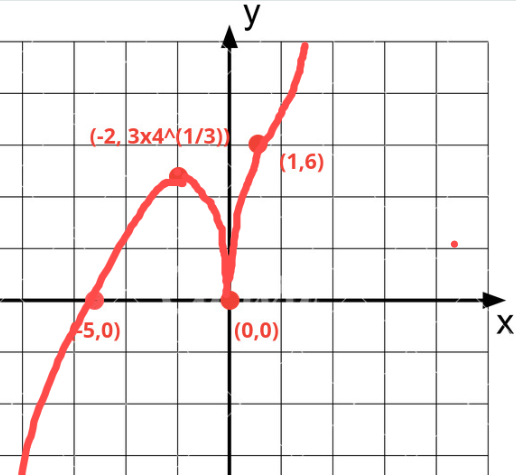
\includegraphics[width=0.5\textwidth]{../img/img_Lista3/p2_36.png}
\end{figure}
\end{itemize}

Comparando con utilidad gráfica:
\begin{figure}[H]
\centering
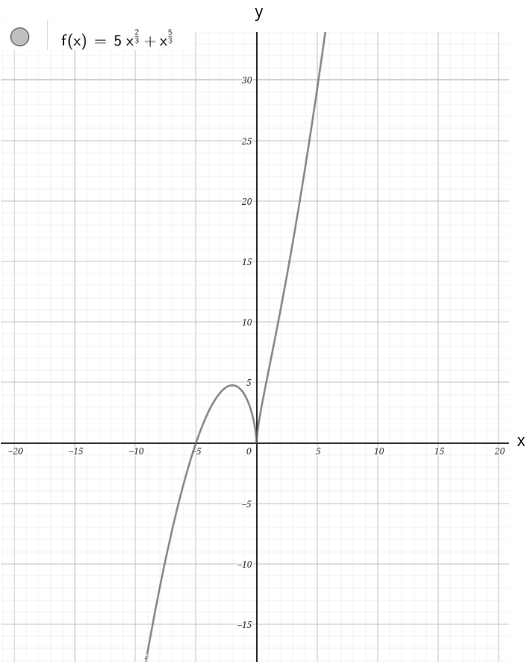
\includegraphics[width=0.85\textwidth]{../img/img_Lista3/p3_36.png}
\end{figure}



% 54 -------------------------------------------------------------------------------------------------------------
\subsection{Ejercicio 54} Flores Morán Julieta Melina \\

Utilizando la regla de L'Hôpital se puede verificar que
\begin{align*}
  \lim_{x \to +\infty} \frac{e^x}{x}=+\infty && \lim_{x \to +\infty} \frac{x}{e^x}=0 && \lim_{x \to -\infty} xe^x=0
\end{align*}
En estos ejercicios: (a) Utilice estos resultados, según sea necesario, para encontrar los límites de $f(x)$ cuando $x\rightarrow +\infty$ y cuando $x\rightarrow -\infty$. (b) Dibuje una gráfica de $f(x)$ e identifique todos los extremos relativos, puntos de inflexión y asíntotas (según corresponda). Comprueba tu trabajo con una utilidad gráfica.
\[
f(x)=x^3e^{x-1}
\]
(a)\\

\[
 \lim_{x \to +\infty}  x^3e^{x-1} = \lim_{x \to +\infty}  x^3  \lim_{x \to +\infty} e^{x-1}  = +\infty \cdot +\infty = +\infty
\]
\[
\lim_{x \to -\infty}  x^3e^{x-1} = \lim_{x \to -\infty}  xe^{x} (x^{2}e^{-1}) =  \lim_{x \to -\infty} xe^{x} \cdot \lim_{x \to -\infty} x^{2}e^{-1} = 0 \cdot \lim_{x \to -\infty} x^{2}e^{-1} = 0
\]
 (b) \\
 \textbf{Extremos relativos:}
 Los extremos relativos son puntos donde la derivada se iguala a 0 y cambia de signo.
 
\begin{align*}
  f'(x)
  &= \frac{d}{dx} \left[x^3e^{x-1} \right]\\
  &= x^{3} \frac{d}{dx} (e^{x-1}) + e^{x-1}  \frac{d}{dx} (x^3)\\
  &= x^{3} (e^{x-1}) + e^{x-1}(3x^2)\\
  &= e^{x-1} ( x^{3}  + 3x^2 )\\
  &= e^{x-1} x^2(x+3)  \\
\end{align*}
Ahora podemos igualar:
\[
f'(x) = x^2(x+3) = 0  
\]
\[
\iff
\]
\[
x= 0 \text{ o } x = -3
\]
Al evaluar los puntos
\[
f(0)=0^3e^{0-1} = 0
\]
\[
f(-3)=(-3)^3e^{-3-1} = (-27)e^{-4} = -0.4945
\]
Por esto los puntos estacionarios son (0,0) y (-3, -0.4945). Y podemos evaluar si tenemos extremos relativos.
 \begin{table}[H]
    \centering
    \begin{tabular}{c|c}
      \hline
      Intervalo & $f'(x) = e^{x-1} x^2(x+3)   $  \\
      \hline
      $(-\infty,-3)$ & -  \\
      $(-3,0)$ & +  \\
      $(0,+\infty)$ & + \\
      \hline
    \end{tabular}
 \end{table}
 Ya que en -3 la derivada va de negativa a positiva, hay un extremo relativo, específicamente hay un mínimo relativo en este punto. \\
\textbf{Puntos de inflexión:}\\
 Los puntos de inflexión son puntos donde la segunda derivada se iguala a 0 y la concavidad cambia.
\begin{align*}
  f''(x)
  &= \frac{d}{dx} \left[ e^{x-1} ( x^{3}  + 3x^2 )   \right]\\
  &=  e^{x-1} \frac{d}{dx}( x^{3}  + 3x^2 ) +  ( x^{3}  + 3x^2 ) \frac{d}{dx} (e^{x-1}) \\
  &=  e^{x-1} ( 3x^{2}+ 6x ) +  ( x^{3}  + 3x^2 ) (e^{x-1}) \\
  &=  e^{x-1} ( 3x^{2}+ 6x  +   x^{3}  + 3x^2 ) \\
  &=  e^{x-1} ( 6x^{2}+ 6x  +   x^{3} )\\
  &=  e^{x-1} x ( 6x+ 6  +   x^{2} ) 
\end{align*}
Ahora podemos igualar:
\[
f''(x) = e^{x-1} x ( 6x+ 6  +   x^{2} )  = 0 
\]
\[
\iff
\]
\[
 x  = 0
 \]
 o
 \[
( 6x+ 6  +   x^{2} )  = 0  \iff x = -3 \pm \sqrt{3}
 \]
 Evaluando los puntos:
 \[
f(-3+ \sqrt{3}) = (-3 + \sqrt{3})^3e^{(-3 + \sqrt{3})-1} = -0.21103
\]
 \[
f(-3 - \sqrt{3}) = (-3 - \sqrt{3})^3e^{(-3 - \sqrt{3})-1} = -0.34433
 \]

 \begin{table}[H]
    \centering
    \begin{tabular}{c|c|c}
      \hline
      Intervalo & $f''(x) = e^{x-1} x ( 6x+ 6  +   x^{2} )$ & concavidad hacia  \\
      \hline
      $(-\infty,-3-\sqrt{3})$ & - & abajo  \\
      $(-3-\sqrt{3}, -3+\sqrt{3})$ & + & arriba  \\
      $(-3+\sqrt{3}, 0)$ & - & abajo  \\
      $(0,+\infty)$ & +arriba \\
      \hline
    \end{tabular}
 \end{table}
  Entonces los  puntos de inflexión son :(0,0), $(-3+ \sqrt{3},-0.21103 ) ~y~ (-3 - \sqrt{3},  -0.34433 ).$
 \\\textbf{Asíntotas:}\\
 -Verticales: No hay ya que la función esta definida para todos los reales. \\
 -Horizontales: Como se vio al evaluar los límites, existe una en y= 0 cuando $x \rightarrow - \infty$ \\


 Con esta información podemos graficar la función de esta forma.\\
\begin{figure}[H]
\centering
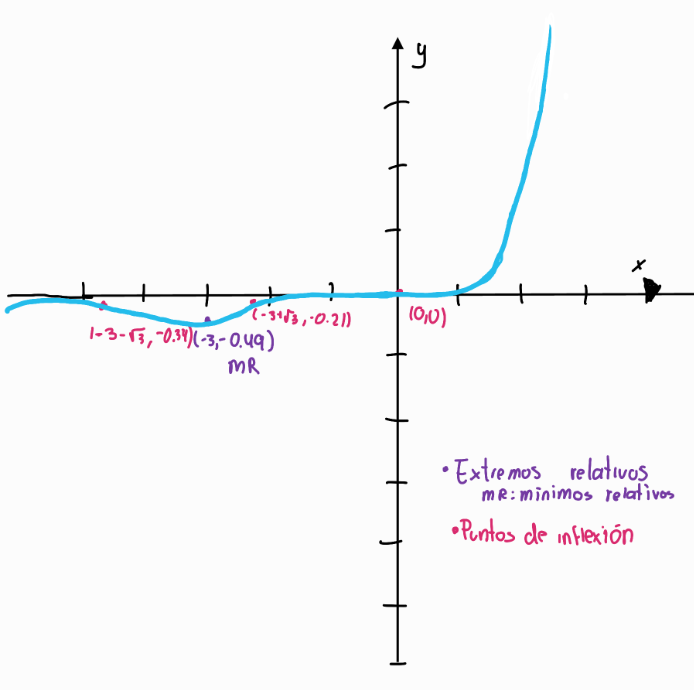
\includegraphics[width=0.4\textwidth]{../img/img_Lista3/54_1.png}
\end{figure}

Y comparando con una utilidad gráfica, obtenemos lo siguiente:
\begin{figure}[H]
\centering
 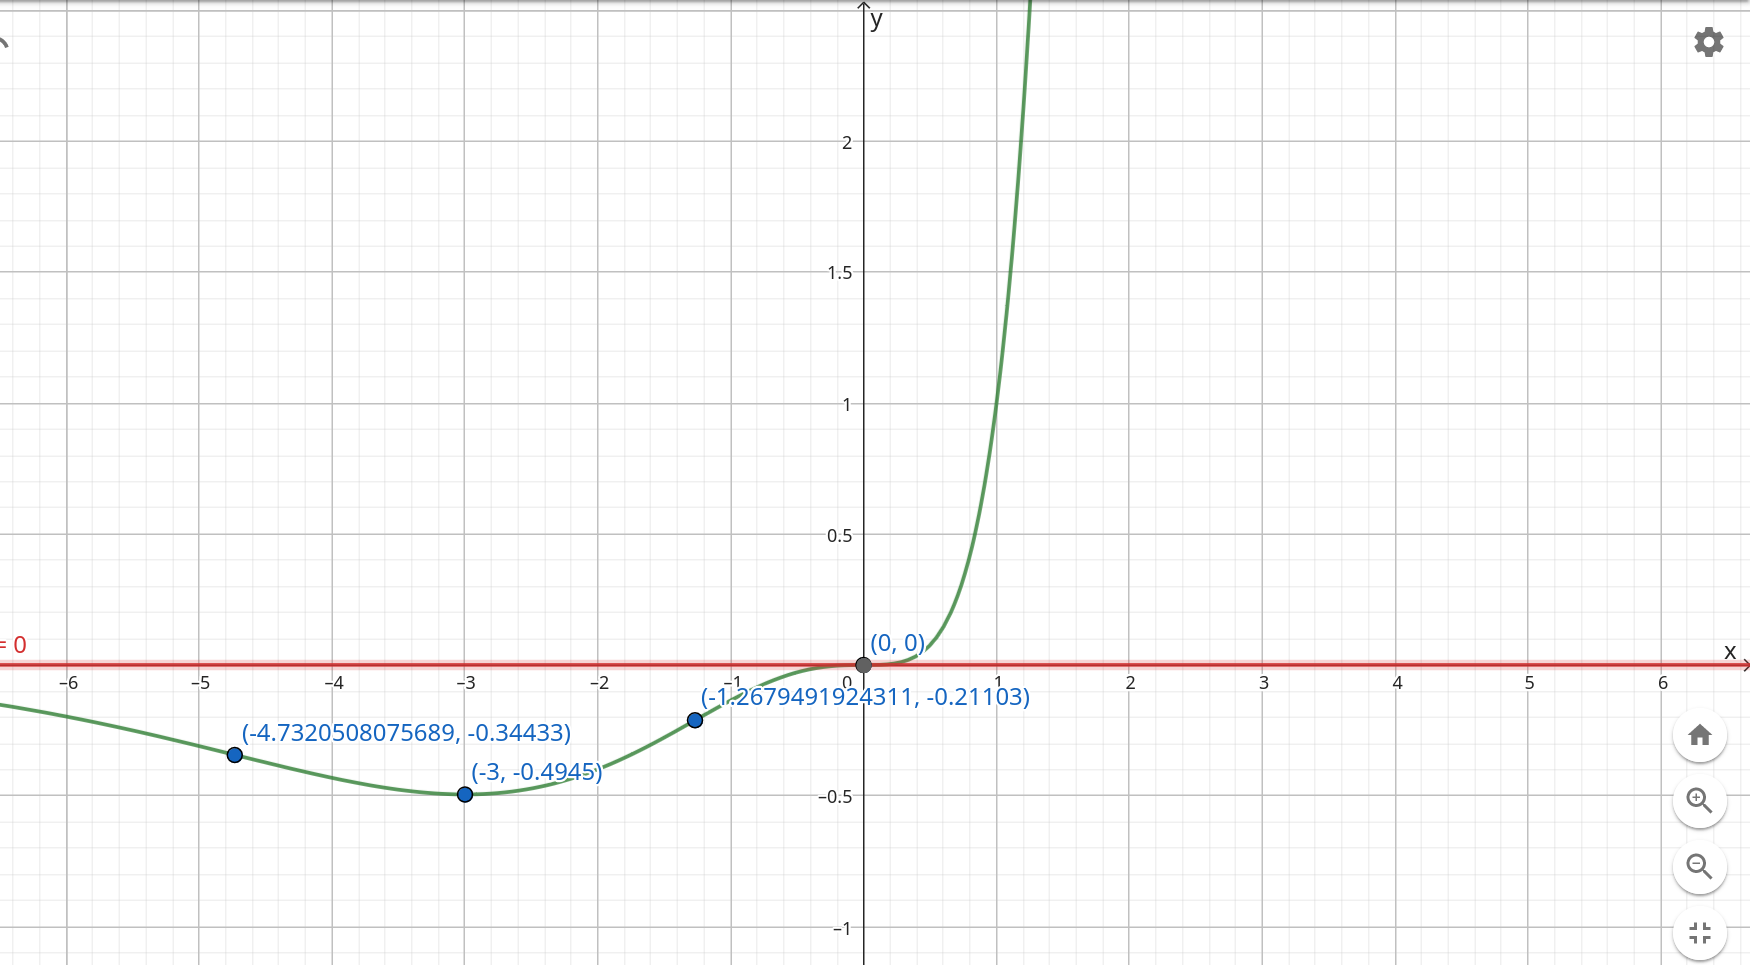
\includegraphics[width=0.4\textwidth]{../img/img_Lista3/54_2.png}
\end{figure}

 % 70 -------------------------------------------------------------------------------------------------------------
\subsection{Ejercicio 70} name \\

La figura adjunta muestra una gráfica generada por computadora del polinomio $y = 0.1x^5 (x + 1)^2$ usando una ventana de visualización de $[−2, 1.5] \times [−0.2, 0.2]$. Demuestre que la elección de la escala vertical hizo que la computadora pasara por alto características importantes de la gráfica. Encuentra las características que faltaron y haz tu propio boceto del gráfico que muestra las características que faltan.
\begin{figure}[H]
\centering
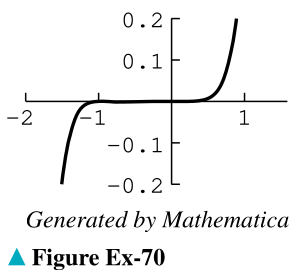
\includegraphics[width=0.4\textwidth]{../img/img_Lista3/2_70.png}
\end{figure}
Primero reescribiremos $f(x)$ como
\begin{align*}
  f(x)
  &=0.1x^5 (x + 1)^2 \\
  &= 0.1x^5(x^2+2x+1)\\
  &= 0.1(x^7+2x^6+x^5)
\end{align*}
Ahora, calculamos $f'(x)$
\begin{align*}
  f'(x)
  &= 0.1(7x^6+12x^5+5x^4)\\
  &= 0.1x^4(7x^2+12x+5)\\
  &=0.1x^4(x+1)(7x+5)
\end{align*}

\begin{table}[H]
  \centering
  \begin{tabular}{c|c|c}
    \hline
    Intervalo & $f'(x) = 0.1x^4(x+1)(7x+5)$ & Conclusión \\
    \hline
    $(-\infty,-1)$ & + & $f$ es creciente \\
    $(-1,-\frac{5}{7})$ & - & $f$ es decreciente \\
    $(-\frac{5}{7},0)$ & + & $f$ es creciente\\
    $(0,+\infty)$ & + & $f$ es creciente\\
    \hline
  \end{tabular}
\end{table}
Dado que el signo de $f'$ cambia de - a + en $x=-\frac{5}{7}$, hay un mínimo relativo allí, y
dado que el signo de $f'$ cambia de + a - en $x=-1$, hay un máximo relativo allí.

Evaluamos
\begin{align*}
  f(x)\vline_{x=-1}
  &=0.1(-1)^5 ((-1) + 1)^2
  =-0.1 (0)^2
  =-0.1\cdot 0
  = 0\\
  f(x)\vline_{x=-\frac{5}{7}}
  &=0.1\left(-\frac{5}{7}\right)^5 \left(\left(-\frac{5}{7}\right) + 1\right)^2
  =-0.1\left(\frac{5}{7}\right)^5 \left(\frac{2}{7}\right)^2\\
  &=-\frac{1}{10} \cdot \frac{3125}{16807} \cdot \frac{4}{49} \\
  &= -\frac{1250}{823543}\\
  & \approx 1.15178 \times 10^{-3}
\end{align*}

$\therefore $ Los puntos críticos son -1, 0 y $-\frac{5}{7}$; en $(-1,0)$ ocurre un máximo relativo y en $\left(-\frac{5}{7}, 1.15178 \times 10^{-3} \right)$ un mínimo relativo.
\begin{figure}[H]
\centering
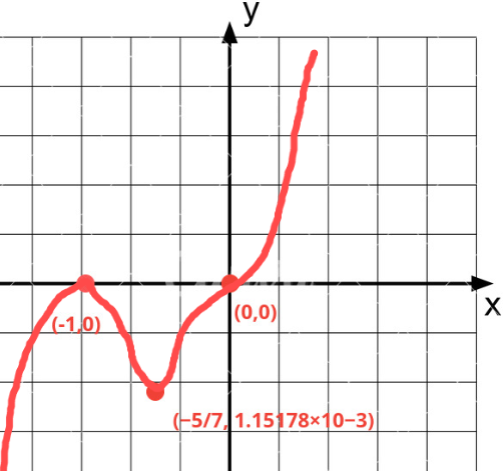
\includegraphics[width=0.6\textwidth]{../img/img_Lista3/2_70_last.png}
\end{figure}

\end{document}
